% !Mode:: "TeX:UTF-8"
%!TEX program  = xelatex

\documentclass[bwprint]{gmcmthesis}
\usepackage{color}
\title{航站楼扩增评估}
\baominghao{4321} %参赛队号
\schoolname{武汉大学}%学校名称
\membera{戴非} %队员A
\memberb{周宇明} %队员B
\memberc{焦冲} %队员C
\begin{document}

 \maketitle

\begin{abstract}
我国航空运输业长期以来处于快速发展的状态,导致航空公司如今面临着一些挑战。其中登机口分配问题是日常生活中最重要的问题,不佳的分配方案会导致资源
浪费以及降低乘客乘坐的满意度,因此解决这个问题主要是为了保证乘客最大便利性的同时最小化所用登机口的数量。国内大量专家学者已对登机口优化问题进行
了研究也在此方面取得了一些研究成果,但在如何保证乘客便利性方面的研究还不够成熟。因此,本文在研究最小化所用登机口的数量的基础上,针对旅客的便捷性
(总体最短流程时间以及紧张度)进行详细分析。


问题1主要涉及\textcolor{red}{数学的最优化处理问题},对于题目所提供的信息,针对20号的数据进行变量定义与组合,建立航班信息与登机口数量之间非
线性数学模型。通过离散化的思想,结合深度优先搜索的算法得到最少使用登机口数量,使得耗费的成本最低。



\keywords{航站楼\quad  登机口\quad   乘客满意度\quad  动态规划模型}
\end{abstract}

\pagestyle{plain}

%目录 不推荐加
\tableofcontents

\section{问题重述}

\subsection{引言}

随着经济的发展,旅游成为了一种大部分现代人的一种生活娱乐方式,传统的交通方式已无法满足人们的需求。近年来乘机旅游已经成为了一种普遍的旅游方式,
这也使得以往的机场资源配置跟不上日益增大的交通需求,其中最为关键的是登机口的合理分配,原来的机场往往根据自身的经验进行登机口的分配和调度,
使得登机口航班组合没有达到最优,从而降低了登机口的利用效率。对于中转乘客而言,不合理的调度耗费了他们过多的中转时间,降低了航班的便捷性。
许多研究者针对这一问题进行了详细分析并得到了一些优化的模型,如SLAM和TAAM。本文需要科学地利用建模解决实际中遇到的问题。

\subsection{问题的提出}

\subsubsection{问题的提出内容一}
为了探讨机场新建卫星厅所带来的影响,本文依次提出了如下问题:

(1)只考虑航班-登机口的分配。建立数学优化模型,尽可能多地分配航班到合适登机口,并且在此基础上最小化被使用登机口地数量,且不需要考虑中转
乘客的换乘。

(2)在问题一的基础上,最小化中转旅客的总体最短流程时间,并在此基础上最小化使用登机口数量,且无需考虑乘坐捷运和步行时间。

(3)考虑中转旅客的换乘时间,并最小化换乘乘客总体紧张度,且在此基础上最小化登机口数量。


\section{模型的假设}
模型假设:
\begin{itemize}
\item 假设收集到的数据都具有真实性和代表新,可以作为各种计算的依据;
\item 假设航班能按时出发和达到;
\item 问题一只考虑航班—登机口分配;
\item 问题二不考虑乘客乘坐捷运和步行时间;
\item 假定临时机位数量无限定;
\item 假定航班的登机口是先到先得
\item 假定在20日第一趟航班到达之前机场为空的。
\item 假定航站楼T和卫星厅S同时使用
\end{itemize}

\section{符号说明}

\begin{tabular}{cc}
 \hline
 \makebox[0.4\textwidth][c]{符号}	&  \makebox[0.5\textwidth][c]{意义} \\ \hline
 Pi	    & 当前到达飞机  \\ \hline
 Gw	    & 登机口权值参数  \\ \hline
 Gs	    & 当前空闲可停登机口  \\ \hline
 Gu     & 当前未开启登机口 \\ \hline
 Gn     & 当前已使用登机口 \\ \hline
 K      & K阶段 \\ \hline
 K+1    & K+1 \\ \hline
$S_{k}$   & 第K阶段状态 \\ \hline
$U_{k}$   & 第K阶段决策 \\ \hline
$U_{k+1}$ & 第K+1阶段状态 \\ \hline



\end{tabular}

\section{问题分析}
合理的利用登机口,不仅可以为乘客提供良好的乘机体验,还可以为航空公司节约了资源成本。传统的登机口的分配方式有很多不足,
所以如何建立起新的登机口分配方式引起了人们的广泛关注。\textcolor{red}{本文就这一问题建立了数学模型},分析了改良后的效果。
通过分析20号当天所有航班的时刻图,得到如下图1所示的信息:
\begin{figure}[!h]
\centering
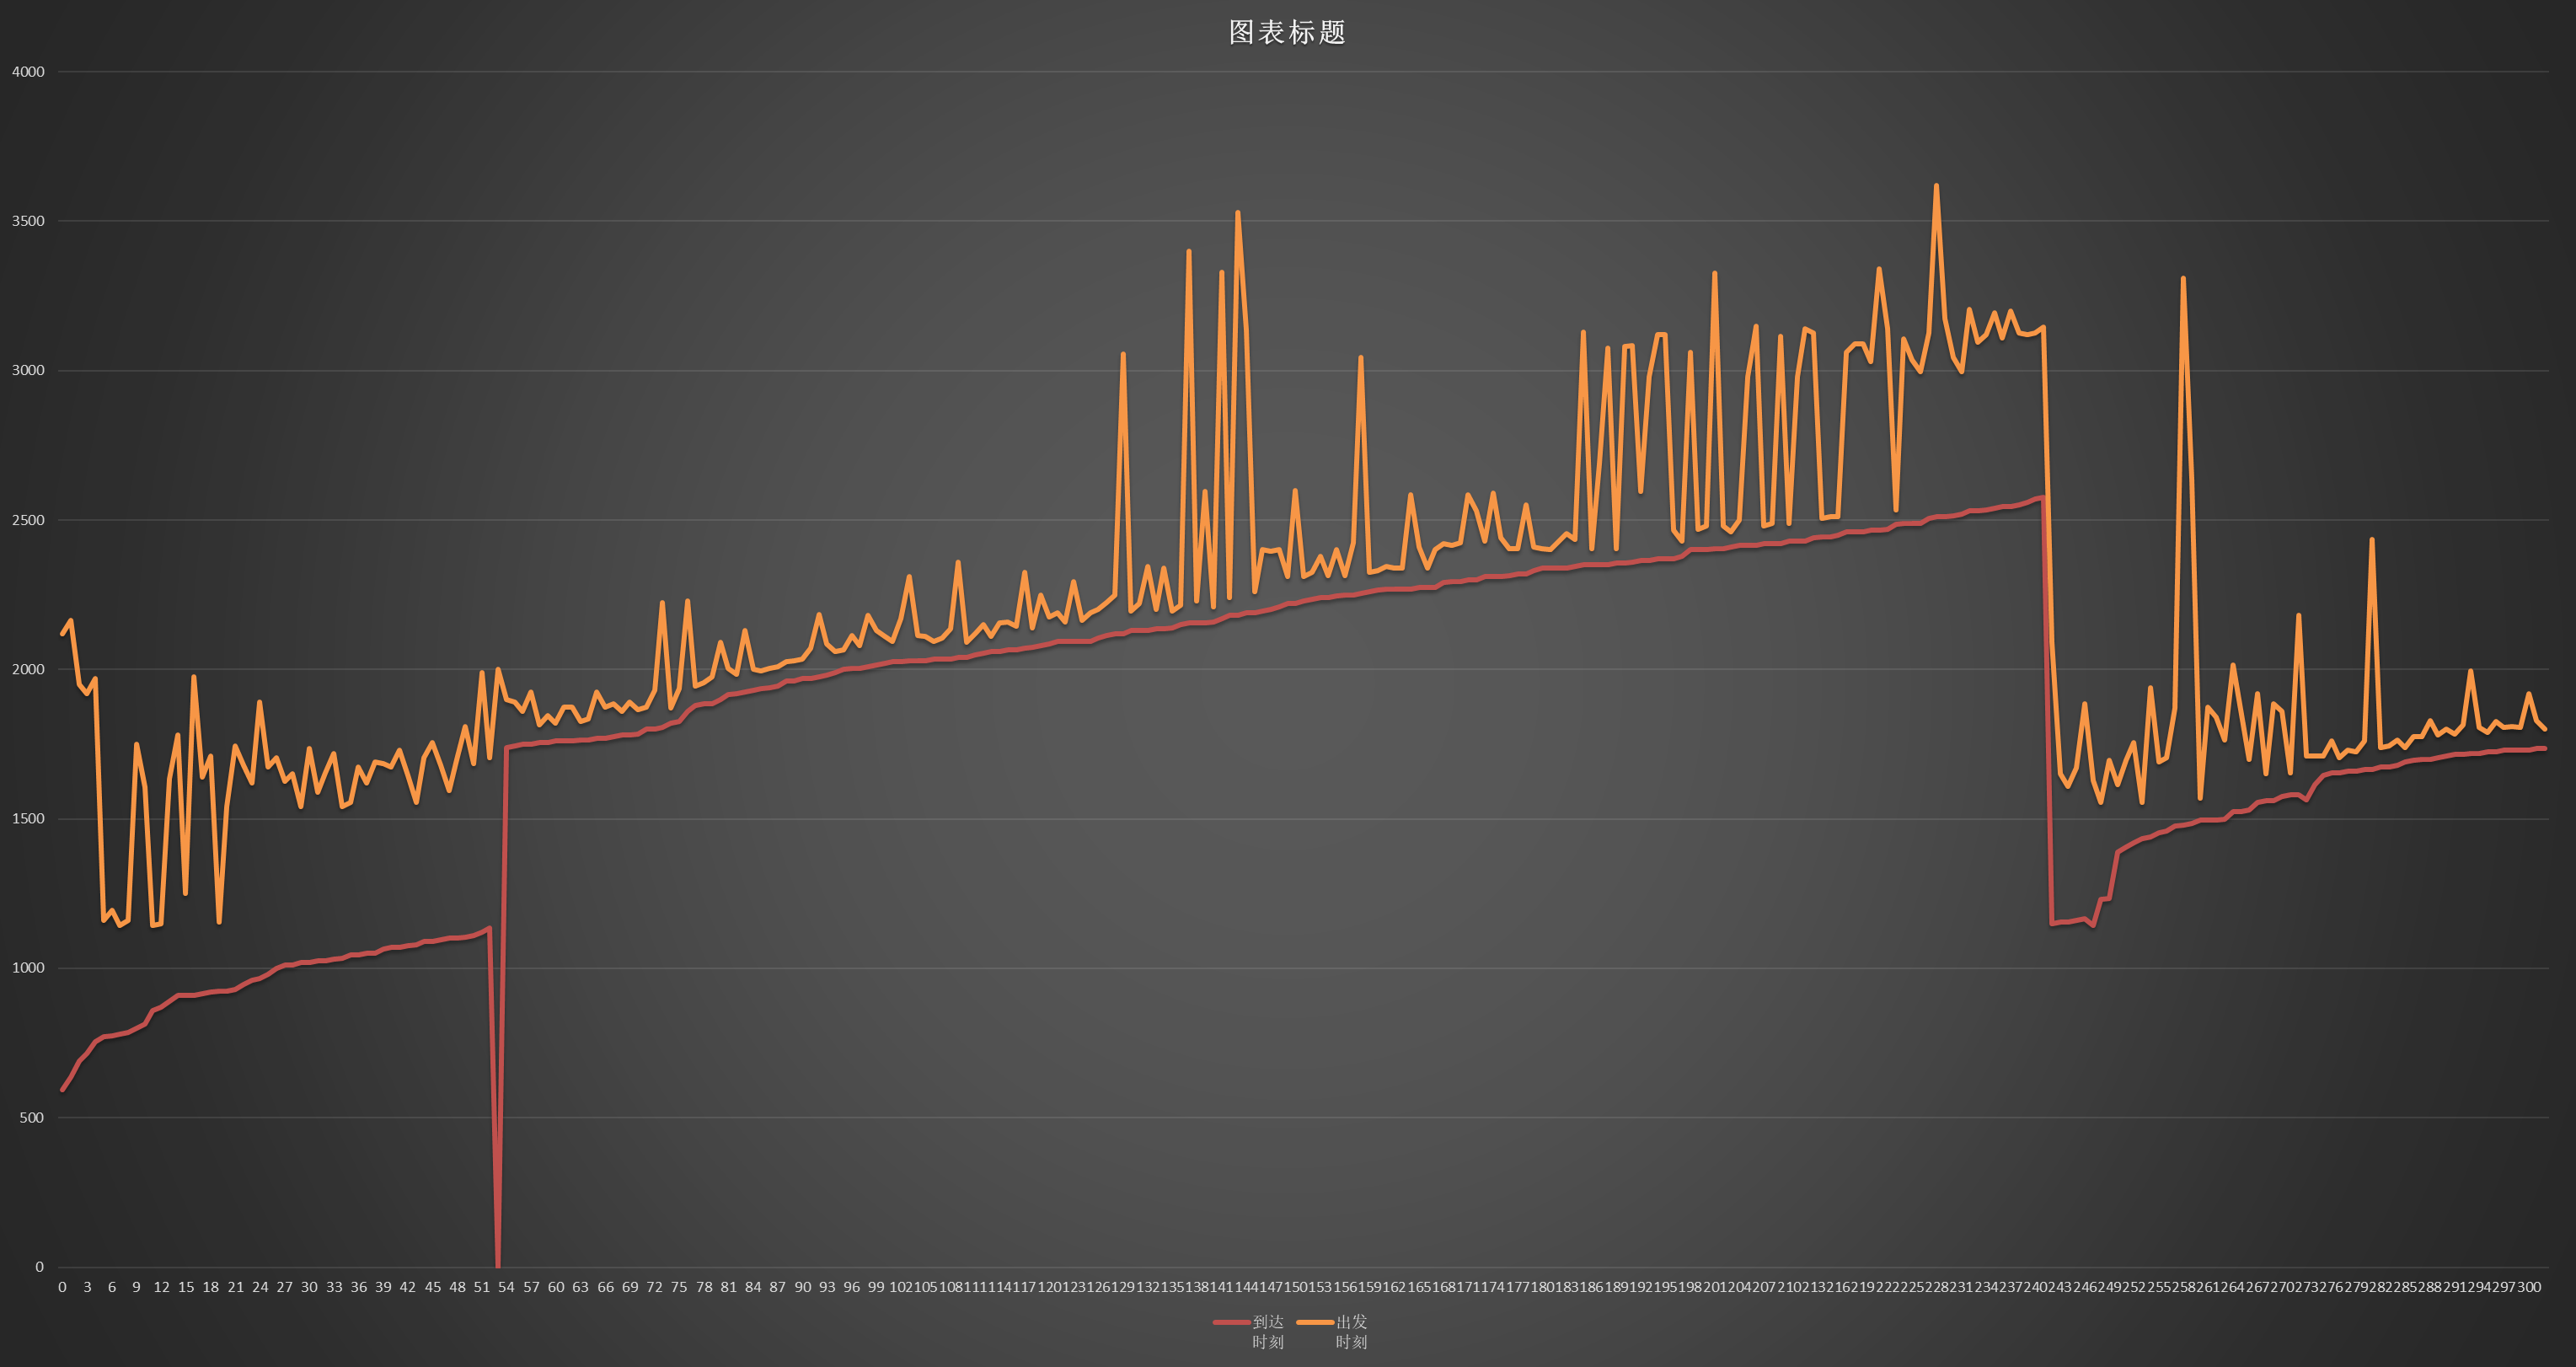
\includegraphics[width=.7\textwidth]{Figure1.png}
\caption{
横坐标代表航班的班次,纵坐标代表航班到达或起飞的时刻,初始时刻为20号最早航班时间。}
\end{figure}

同时,登机口的属性介绍如下图2所示
\begin{figure}[!h]
\centering
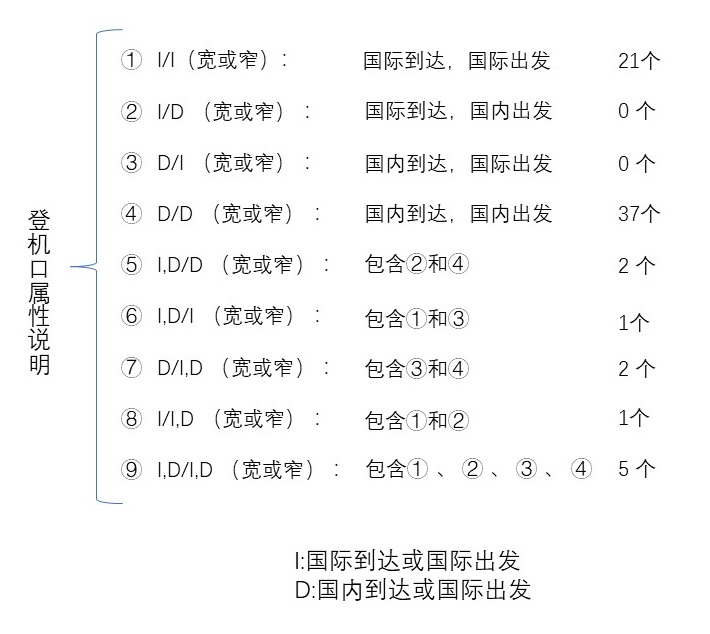
\includegraphics[width=.9\textwidth]{Figure2.jpg}
\caption{登机口属性介绍}
\end{figure}
\subsection{问题一分析}
问题1要求建立出能保证在尽可能多地分配航班到合适的登机口的同时,最小化登机口的数量。对于本文所提供的20号航班数据,某时刻
登机口的状态和最邻近45分钟之前的登机口的状态有关,故采用模型一的动态规划思想建立出动态转移方程,最后得到最小化登机口数量。
然后采用深度优先搜索得到的精确的结果进行模型的检验,发现能较好的保证结果的正确性。

由于登机口数据表格可知,不同登机口属性配置皆不相同,某些登机口可以使用多种航班的转场。因此,为了得到分配方案,我们采用贪心算法,
按照时间顺序依次处理每一个航班,并赋予不同登机口优先级权值,按照权值的大小,分配对应航班,从而获取登机口使用最少分配方案。


\subsection{问题二分析}

\subsection{问题三分析}

\section{模型的建立与求解}

\subsection{最小化登机口数量模型}
\subsubsection{动态规划思想的运筹学模型}
动态规划算法一般用来求解具有某种最优性质的问题。这类问题中往往有
许多可行解,需要从这些子问题的解得到原问题的解。
此模型多阶段决策问题,这类问题的活动过程能够分为多个相互联系的阶段,在每一个阶段都需要采取相应措施,一个阶段的决策被定义以后
会影响下一个阶段的决策。最终把各个阶段的决策结合起来构成一个决策序列,称为策略。各个阶段不同的决策导致了有许多策略供我们选择,
每个策略的活动效果可以用数量来确定。此问题要求在选择的那些策略中间,选取一个最优策略以达到最好的效果。 此题适用于用此运筹学模型求解。
相对应的动态转移方程为
\begin{equation}
S_{k+1}=U_{K}\left ( S_{K} \right )
\end{equation}

\subsubsection{带权值的贪心算法模型}
通过对登机口数据进行统计和分析,得到登机口属性类型一共为七种,分别为图2中的(1)(4)(5)(6)(7)(8)(9),其数量依次是:21,37,1,1,2,2,5。因此,
在每次对航班进行选择时,为了保证后续航班的停靠,我们采用如下表所示的权值设计:

\begin{tabular}{c|c|c}
  \hline
  \makebox[0.3\textwidth][c]{属性抽象类}	&  \makebox[0.3\textwidth][c]{登机口数量} &  \makebox[0.3\textwidth][c]{权值分配} \\ \hline
  I/I	     & 21  &  \\ \hline
  D/D	     & 37  &  \\ \hline
  I,D/D	   & 1   &  \\ \hline
  I,D/I	   & 1   &  \\ \hline
  D/I,D    & 2   &  \\ \hline
  I/I,D    & 2   &  \\ \hline
  I,D/I,D  & 5   &  \\ \hline
\end{tabular}

带权值的贪心算法模型流程如下图3所示
\begin{figure}[!h]
\centering
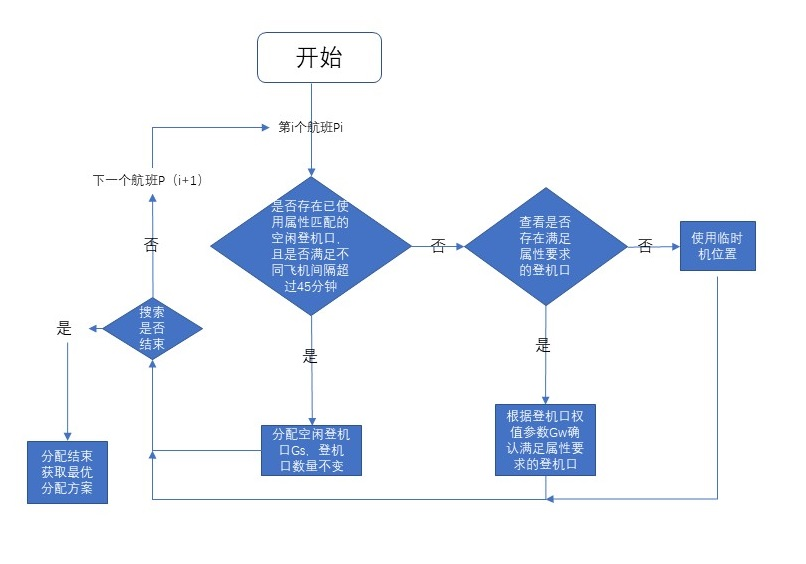
\includegraphics[width=.9\textwidth]{Figure3.jpg}
\caption{带权值贪心算法流程图}
\end{figure}
如上图所示,整个算法的流程主要分为三步:
begin{itemize}
\item \textbf{Step1}-对20号所有航班的到达时间进行排序,从第一个航班$P_{i}$开始,根据属性条件以及权值参数$Gw$确认停放登机口,并将使用的
登机口数量$G_{n}$+1
\item \textbf{Step2}-处理航班$P_{i+1}$,遍历空闲航班$G_{s}$, 若存在满足航班属性要求的登机口,则选取权值最高的登机口,$G_{n}$不变。否则
查看剩余未开放的登机口$Gu$,若存在满足航班属性要求的登机口,则开放此登机口用于停放,$G_{n}$+1。如果皆找不到满足条件的登机口,则开放临时
机位用于停靠,$G_{n}$不变。
\item \textbf{Step3}-若处理完所有航班,则输出$G_{n}$,否则重复\textbf{Step2}。

\end{itemize}




\subsection{对数据应用模型并求解}
\subsubsection{单独考虑最小化登机口数量的求解}
(1)动态规划思想的模型

先将登机口的属性抽象为II-W,II-N,ID-W,ID-N,DI-W,DI-N,DD-W,DD-N八种类型,然后根据题目中所给表中的数据将每个航班到达时刻
当前八种类型的正在使用数目和空闲数目更新,统计八种类型数目的总和并将每个时刻类型对应数目存入Excel表以作后续分析。模型需要
对python筛选出的303次航班数据进行遍历,每次需要更新二维数组,并将每次结果存入临时数组。算法主要时间耗费在遍历上,复杂度为O(n),
模型的实现具有可行性,耗费的时间不长。
具体代码见附录


\subsection{考虑中转旅客最短流程时间的求解}
\subsection{考虑中转旅客的换乘时间的求解}
\section{模型的评价}
\subsection{模型的优点}

\subsection{模型的缺点}
\subsection{模型的改进}
\subsection{模型的推广}

\bibliographystyle{gmcm}
\bibliography{example}


\newpage
%附录
\appendix
%\setcounter{page}{1} %如果需要可以自行重置页码。
\section{我的 MATLAB 源程序}
\begin{lstlisting}[language=Matlab]%设置不同语言即可。
kk=2;[mdd,ndd]=size(dd);
while ~isempty(V)
[tmpd,j]=min(W(i,V));tmpj=V(j);
for k=2:ndd
[tmp1,jj]=min(dd(1,k)+W(dd(2,k),V));
tmp2=V(jj);tt(k-1,:)=[tmp1,tmp2,jj];
end
tmp=[tmpd,tmpj,j;tt];[tmp3,tmp4]=min(tmp(:,1));
if tmp3==tmpd, ss(1:2,kk)=[i;tmp(tmp4,2)];
else,tmp5=find(ss(:,tmp4)~=0);tmp6=length(tmp5);
if dd(2,tmp4)==ss(tmp6,tmp4)
ss(1:tmp6+1,kk)=[ss(tmp5,tmp4);tmp(tmp4,2)];
else, ss(1:3,kk)=[i;dd(2,tmp4);tmp(tmp4,2)];
end;end
dd=[dd,[tmp3;tmp(tmp4,2)]];V(tmp(tmp4,3))=[];
[mdd,ndd]=size(dd);kk=kk+1;
end; S=ss; D=dd(1,:);


 \end{lstlisting}


\end{document}
